\subsection{High throughput binding affinity calculator Workflow}

% BAC uses the Ensemble Toolkit to create a high-throughput workflow which we
% refer to as HTBAC. 

HT-BAC is a workflow system that uses RADICAL-Cybertools to implement ESMACS,
and similar protocols such as TIES. These workflows consist of pipelines with
stages comprised of heterogeneous tasks. For example equilibration and
production, followed by post processing steps. 

Although ESMACS and TIES methods are similar at a high-level, viz., they are
comprised of concurrent, multi-stage pipelines with synchronization (Fig.
5(R)), The different protocols supported by HTBAC differ in the details of the
pipelines, stages and synchronization.

HTBAC uses the EnTK API to express these workflows. RADICAL-Cybertools
provides advanced resource management capabilities and, thereby deliver the
necessary high-throughput capabilities required. The framework is generic and
can be simply expanded to run the MBAR protocol. EnTK provides a common API,
execution and programming model to these different methods, and thus will
minimize development effort and complexity.

The Ensemble Toolkit API exposes four components (‘Resource
Handle’, ‘Pipeline’, ‘Stage’, and ‘Task') to the user which express the
application logic of HTBAC. We describe these components for one of the HTBAC
protocols, ESMACS. The ESMACS protocol contains a set of pipelines where each
pipeline contains functions that operate on a given replica. The pattern of
pipelines are identical and describes an ensemble of preprocessing and
simulation stages as shown in figure control-flow.

\begin{figure}[ht]
\centering
  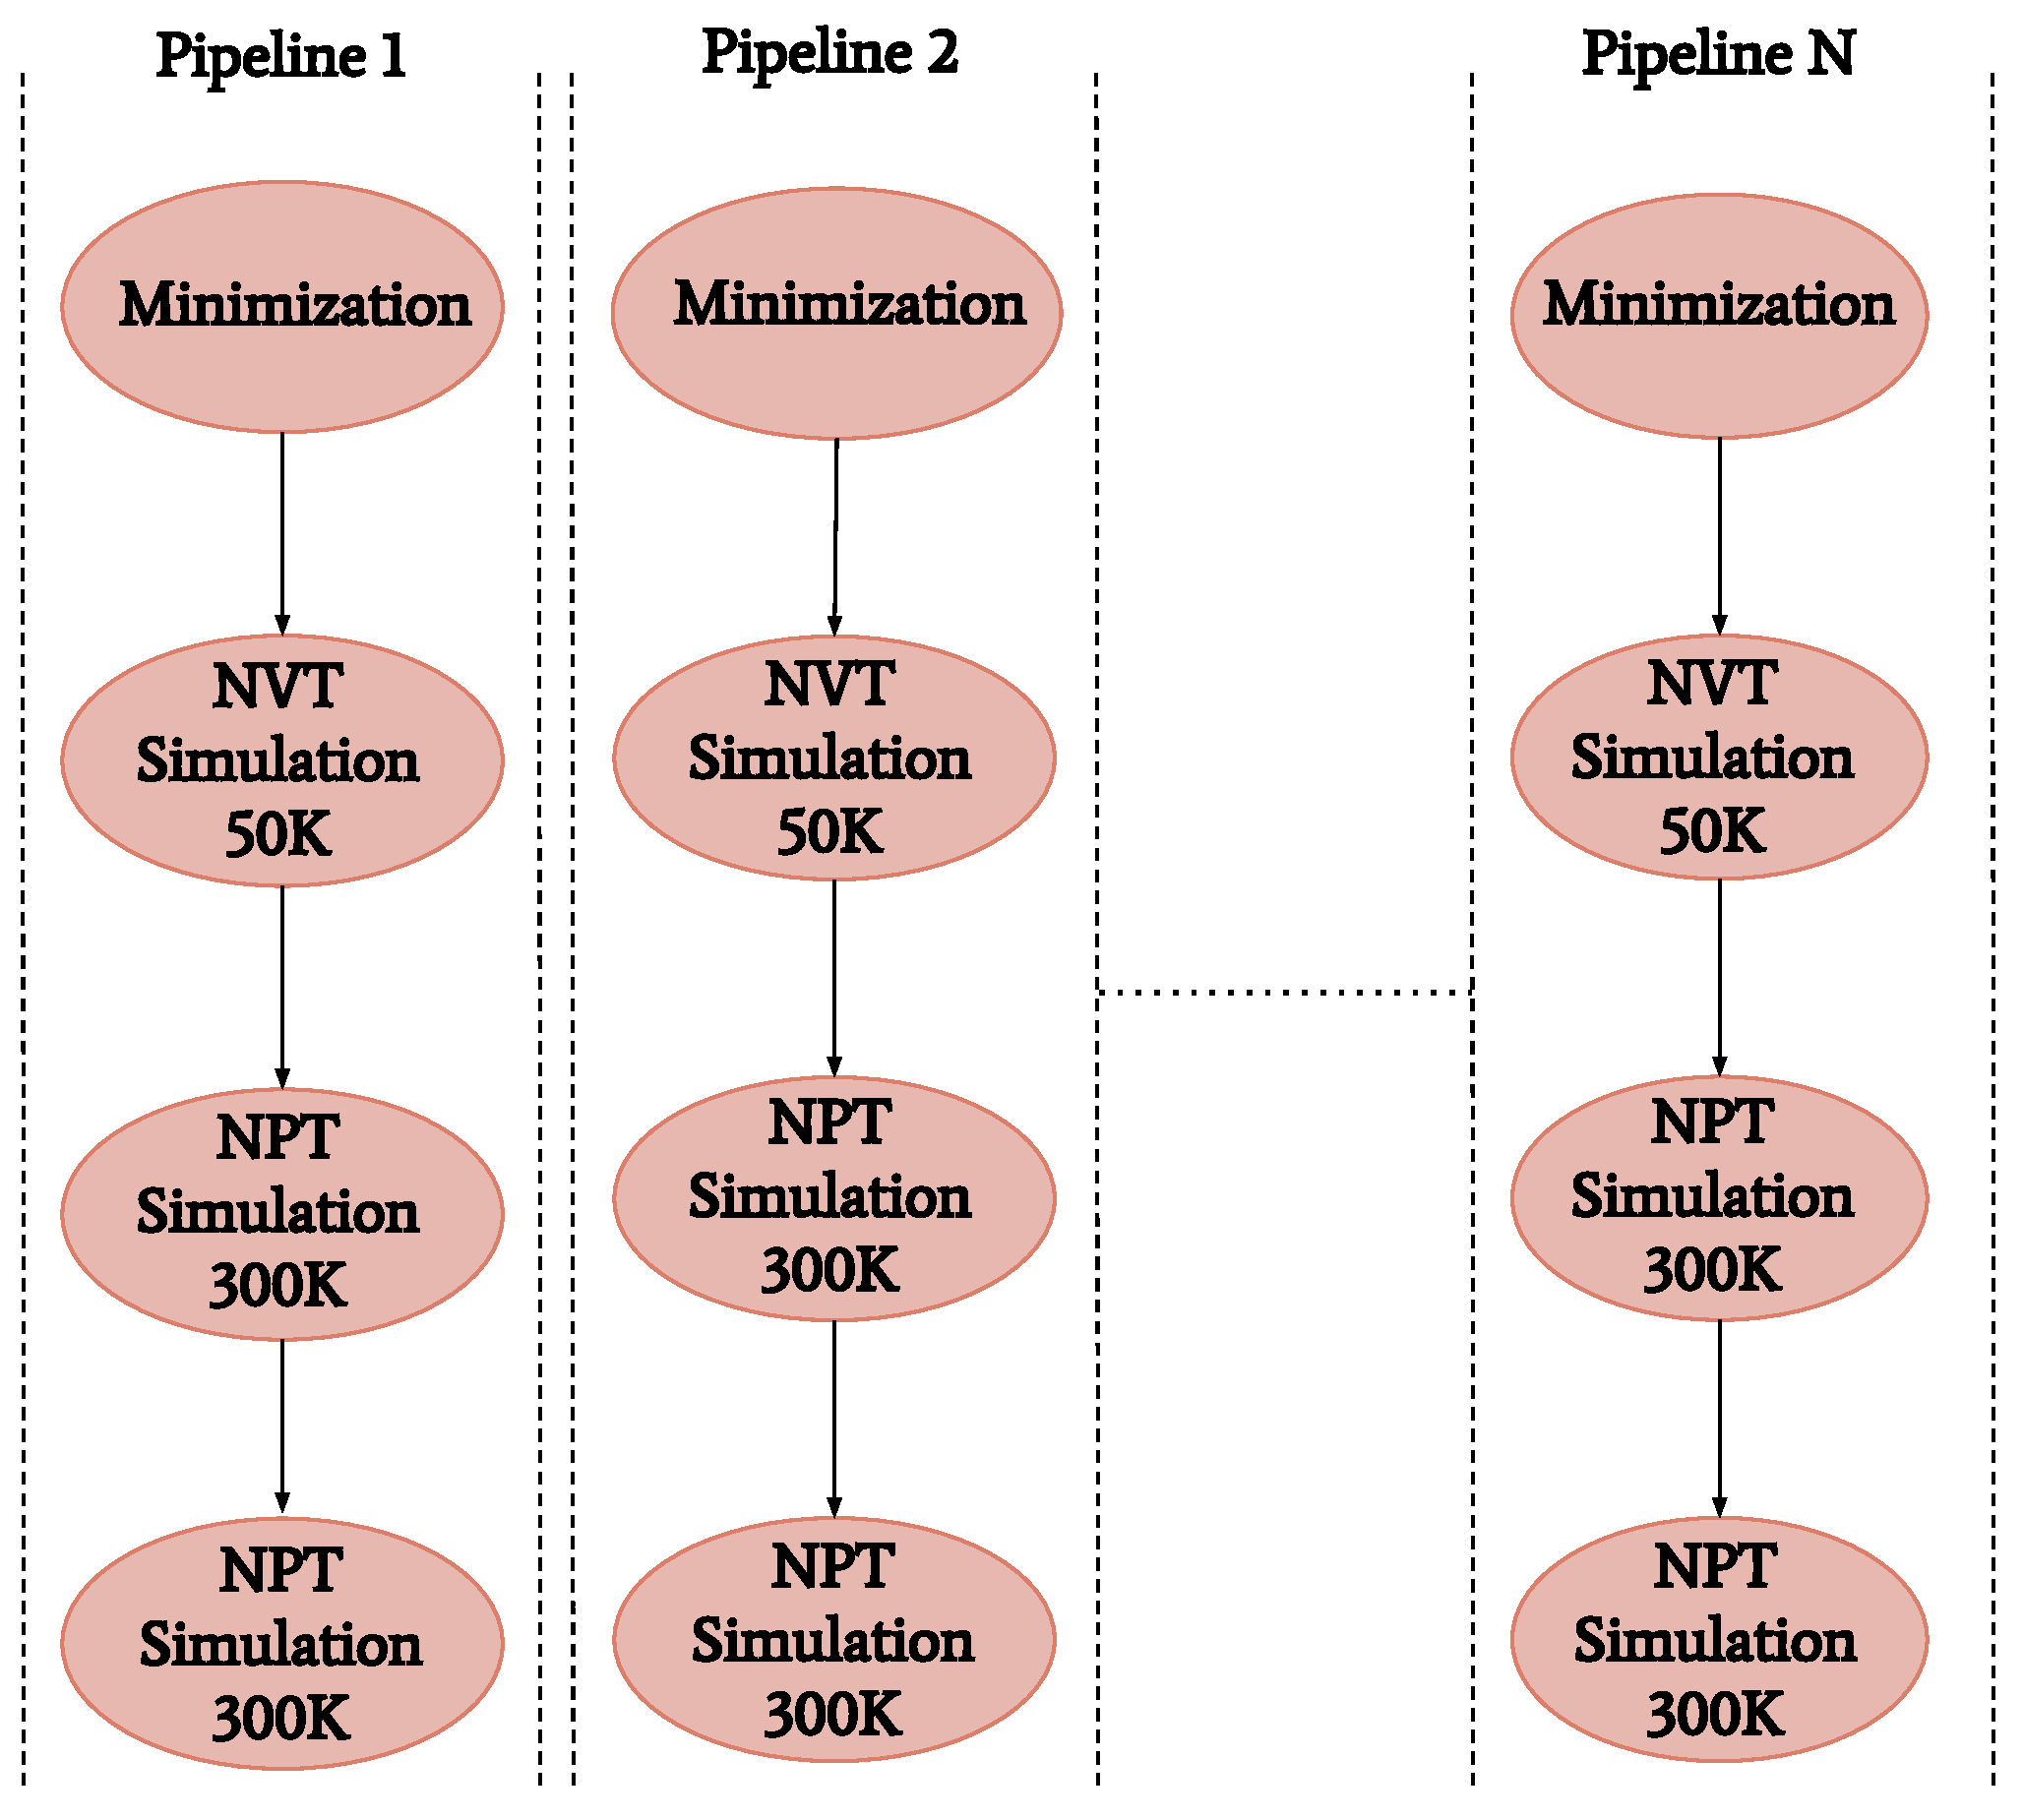
\includegraphics[width=0.5\textwidth]{FIGURES/HT-BAC-NAMD-pipelines-control-flow-only.pdf}
  \caption{\bf ESMACS protocol indicating n-pipelines where each pipeline represents...}
   \label{figure:ESMACS-pipelines}
\end{figure}

%\begin{itemize}
%	\item 1) Untar configuration files
%	\item 2) Preprep
%	\item 3) Minimize with decreasing restraints
%	\item 4) Equilibration: NVT simulation at 50K, with restraints
%	\item 5) Equilibration: NPT simulation at 300K, with decreasing restraints 
%	\item 6) Equlibratin: NPT at 300k, no constraints
%	\item 7) Tarball output files 
%\end{itemize}

Each stage is composed of a single unique task which is described by set of attributes that define the workload parameters such as the location of input files, the number of simulations and the MD engine to run the simulations. The task is appended to a stage and stages are appended to a pipeline to maintain temporal order. The workflow relies on a resource configuration which consists of the details required to use a resource where the application will be executed including runtime, queue, and account details. We capture the integration of the application (ESMACS protocol) and how it interfaces with EnTK in figures ht-bac-rp-integration and entk-htbac-integration. 


\begin{figure}[tb]
\centering
  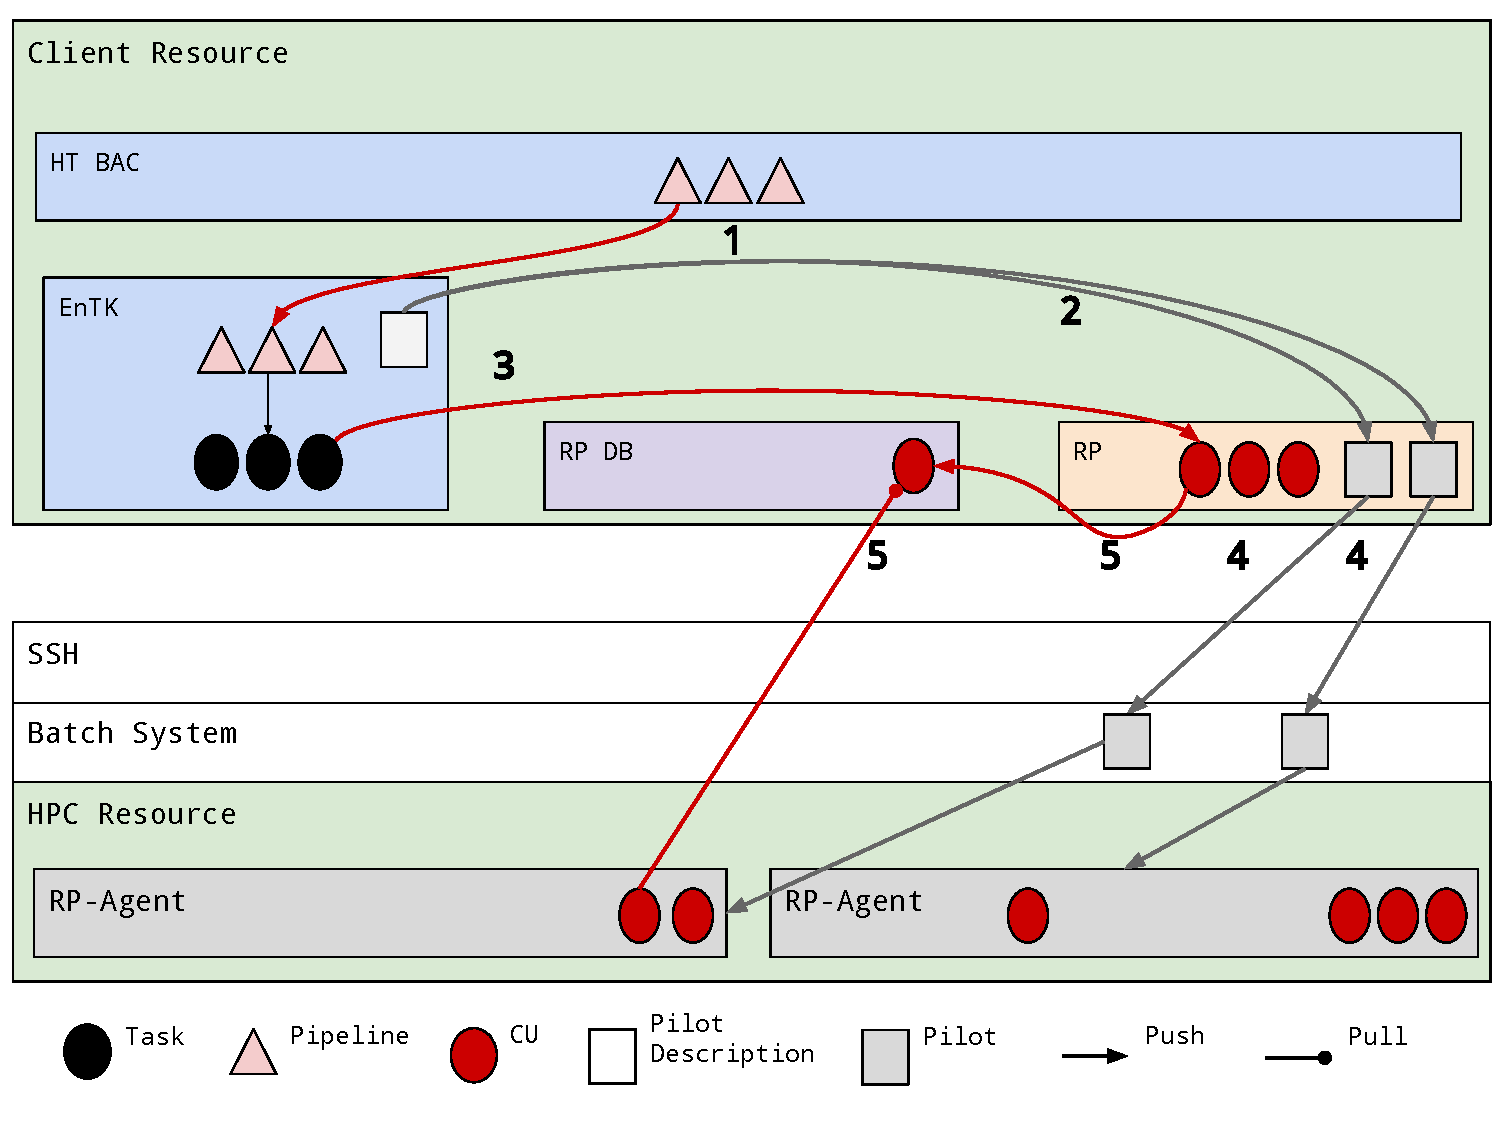
\includegraphics[width=0.5\textwidth]{FIGURES/ht-bac-rp_integration.pdf}
  \caption{\bf Integration between HT-BAC workflow system and EnTK. Numbers indicate the temporal sequence of execution. RADICAL-Pilot (RP) database (DB) can be deployed on any host reachable from the resources.}
   \label{figure:ht-bac_rp}
\end{figure}

\begin{figure}[ht]
\centering
  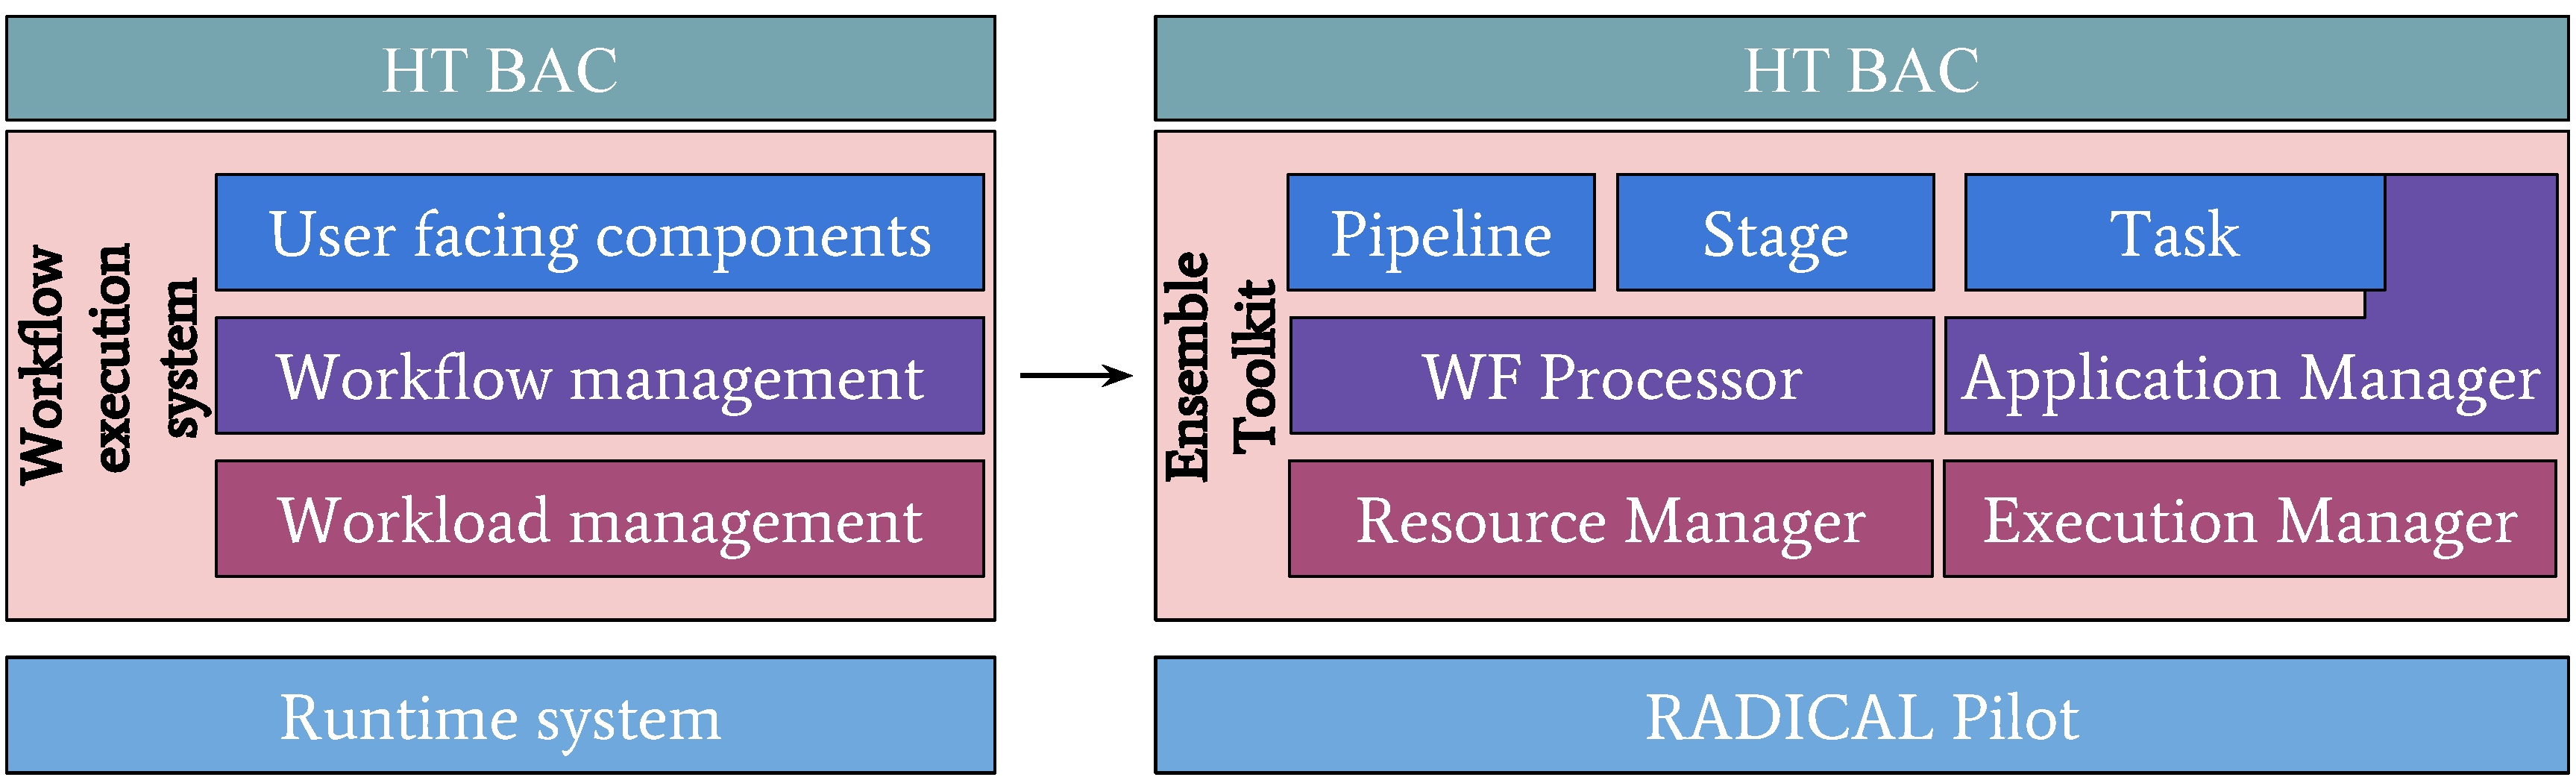
\includegraphics[width=0.5\textwidth]{FIGURES/entk_htbac_integration.pdf}
  \caption{\bf Integration between HT-BAC workflow system and EnTK that shows resource/application managers.}
   \label{figure:ht-bac_entk}
\end{figure}

Add code snippets 

How to express ESMACS and how to execute ESMACS


Remind the reader of the 7 stages of the ESMACS protocol, and how the stages are expressed, and how the pipelines are added 


